% !TeX root = RJwrapper.tex
\title{A Robust Workflow for Forecasting with Bayesian SARIMA Models}
\author{by Daniel Dala and Asael Matamoros}

\maketitle

\abstract{The Box-Jenkins method shows a set of steps to make predictions on time series with ARIMA models using a frequentist approach. In this study we present an adaptation of this method to a Bayesian approach. For the parameter estimation we use Bayesian inference approximating the posterior distribution of the models using Markov Chain Monte Carlo methods. For the model checking, is analysed the behaviour and distribution of the errors that follow an assumption of Gaussian white noise and for the model comparison the differences in the precision of the predictions are measured using cross-validation and comparing the predictions in a test set. Finally, we demonstrate the performance of the proposed methodology on two applications, one forecasting the average monthly temperature in Honduras and one forecasting the monthly closing price in the stock market of Pfizer Inc.}
%
\section{Introduction}
One of the most important applications in time series analysis is prediction, that is, estimating future values that are generally unknown, for this there are different methodologies such as space and state models \citet{rob}, Prophet  \citet{ref2}, neural networks \citet{ref3}, splines \citet{ref4}, Gaussian processes  \citet{ref5}, among others. A very popular class of models for their easy interpretation and high predictive capacity are the SARIMA models \citet{arima,sarima}, but their implementation with real data is complex because selecting the order of the model is a complicated task. Box and Jenkins (1970) proposed a methodology for the proper use of these models, which is based on six iterative stages:\textit{ data visualization, model selection, parameter estimation, model checking, model comparison and forecasting}. This methodology is illustrated in Figure~\ref{fig:Box}.

There are many schemes for the inference process, and in recent years Bayesian inference has become a widely used alternative for data analysis with many applications in economics, physics, chemistry, psychology, among others. Its growing popularity is due to its ability to incorporate external information into the model through a priori distribution, and update beliefs through Bayes' Theorem. This inference approach in practice is very complicated, which is why in recent years the results have been approximated using the Markov Chain Monte Carlo methods  \citet{MCMC}. These methods consist in generating a Markov chain whose stationary distribution is the posterior distribution of the model, there are many procedures to implement these methods, one of the most common is the Monte-Carlo Hamiltoneano, which due to its flexible implementation in the Stan language has been useful in multiple applications \cite{Stan}.

The biggest obstacle when performing an adequate data analysis in a Bayesian approach is that the estimation, checking, and selection procedures used in \citet{boxjen} are not valid in this new approach. propose an extensive and robust methodology called \textit{"Bayesian workflow"}, which presents different tools for an adequate data analysis. This methodology is based on the one proposed by \citet{boxjen}, and it is generalized for any type of modeling that involves a probabilistic inference approach.

The two main problems of the \citet{Aki} method when applied in the analysis of time series are its complex structure, and that some tools are not suitable for data with dependency assumptions, therefore, in this study we present a simplification of the \textit{Bayesian Workflow} with slight variations in some of the tools for their adequate use in time series. Finally, we apply our proposed methodology through two examples. In the first example we predict the average monthly temperature in Honduras with records from 1980 to 2013 obtained from \citet{berkeley}, and a second example analyzing the average monthly closing price of shares in the pharmaceutical company Pfizer with a set of recorded data monthly from 2010 to 2021 obtained from \citet{kaggle}.
%Los dos principales problemas del método de \textit{Gelman, Vehtari et. al. (2020)} al ser aplicados en el análisis de series temporales son su compleja estructura, y que algunas herramientas no son adecuadas para datos con supuestos de dependencia, por lo tanto, en este estudio presentamos una simplificación del \textit{Bayesian Workflow} con ligeras variaciones en algunas de las herramientas para su adecuado uso en series temporales. Finalmente, aplicamos nuestra metodología propuesta mediante dos ejemplos. En el primer ejemplo predecimos la temperatura promedio mensual en Honduras con registros desde el año 1980 hasta el año 2013 obtenido de \citet{berkeley}, y un segundo ejemplo analizando el precio de cierre promedio mensual de las acciones en la empresa farmacéutica Pfizer con un conjunto de datos registrados mensualmente desde el año 2010 hasta el año 2021 obtenidos de \citet{kaggle}.
%	
\section{Preliminaries and notation}
%Para los objetivos de este estudio un proceso estocástico es una colección arbitraria de variables aleatorias $\{Y_1,Y_2, \ldots \}$, y una serie de tiempo o simplemente serie, es una realización o muestra finita $\{y_1,y_2, \ldots , y_n\}$ del proceso. Una propiedad importante a considerar es la estacionaridad, diremos que un proceso $\{y_i\}_{i\in\mathbb{Z}}$ es \textit{estacionario fuerte} si para cualquier colección finita del proceso su distribución conjunta se mantiene constante en el tiempo. Esto es
For the purposes of this study, a stochastic process is an arbitrary collection of random variables $\{Y_1, Y_2, \ldots \}$, and a time series or simply series, it is a realization or finite sample $\{y_1, y_2 , \ldots, y_n \}$ of the process. An important property to consider is stationarity, we will say that a process $\{y_i \}_{i \in \mathbb{Z}}$ is \textit{strong stationary} if for any finite collection of the process its joint distribution holds constant in time. This is
%
$$
F_X(y_{t_1},y_{t_2},...,y_{t_n})=F_X(y_{t_{1+\tau}},y_{t_{2+\tau}},...,y_{t_{n+\tau}}),
$$
%
%para $t\in\mathbb{Z}_+$ con $n\in\mathbb{N}$ y cualquier $\tau\in\mathbb{Z}_+$. Una propiedad menos restrictiva es la estacionaridad débil,  diremos que el proceso $\{y_i\}_{i\in\mathbb{Z}}$ es \textit{estacionario débil} si el proceso tiene una media y varianza constante a través del tiempo, y la  auto-correlación es una función lineal de la diferencia de dos tiempos.
for $t \in \mathbb{Z}_+$ with $n \in \mathbb{N}$ and any $\tau \in \mathbb {Z}_+$. A less restrictive property is weak stationarity, we will say that the process $\{y_i \}_{i \in \mathbb{Z}}$ is \textit{weak stationary} if the process has a constant mean and variance through the time, and the auto-correlation is a linear function of the difference of two times.
%
$$
\mu(t)=\mu \hspace{0.2cm},\hspace{0.2cm} \sigma^2(t)=\sigma^2,\hspace{0.2cm} corr(t,k) = \tau |t - k|.
$$
%
%Para $t,k \in \mathbb{Z}$ y $\tau > 0$. Una serie  $\{y_t\}$ presenta tendencia sobre la media del proceso, si la media  puede representarse como una función en el tiempo $y_t = f(t) + \varepsilon_t$, donde $\{\varepsilon_t\}$ es un proceso con media cero y $f:\mathbb{Z} \to \mathbb{R}$ es una función medible. Para transformar un proceso con tendencia en uno estacionario, aplicamos el operador diferencia
for $t, k \in \mathbb{Z}$ and $\tau> 0$. A series $\{y_t \}$ shows a trend over the mean of the process, if the mean can be represented as a function in time $y_t = f(t) + \varepsilon_t$, where $\{\varepsilon_t \} $ is a process with zero mean and $f:\mathbb{Z} \to \mathbb{R}$ is a measurable function. To transform a process with a trend into a stationary one, we apply the difference operator
%
\begin{equation}\label{eq: diff}
	\nabla y_t=y_t-y_{t-1}.
\end{equation}
%
%Para un proceso $y$ con tendencia lineal, el proceso $\nabla y$ obtenido en la ecuación~\ref{eq: diff} es estacionario. La ciclicidad en una serie, implica múltiples oscilaciones periódicas en la media del proceso, un caso particular es la estacionalidad, esta sucede cuando la serie presenta una oscilación periódica constante  de periodo $m$ en la media. Para transformar un proceso estacional en uno estacionario, aplicamos el operador diferencia estacional
For a process $y$ with a linear trend, the process $\nabla y $ obtained in the equation~\ref{eq: diff} is stationary. The cyclicality in a series implies multiple periodic oscillations in the mean of the process, a particular case is seasonality, this happens when the series presents a constant periodic oscillation of period $m$ in the mean. To transform a seasonal process into a stationary one, we apply the seasonal difference operator
%
\begin{equation}\label{eq: diff_est}
	\nabla_m y_t=y_t-y_{t-m}.
\end{equation}
%
%Donde $m$ es un entero positivo que representa el  periodo de la serie, y para una serie $y$ con estacionalidad,  el proceso $\nabla_m y$ obtenido en la ecuación~\ref{eq: diff_est} es estacionario. Es importante recalcar que las series con tendencia o estacionalidad son no estacionarias, por los efectos de modelado, es necesario trabajar con procesos estacionarios.  Un ejemplo de procesos estacionarios son los ruidos blancos, una colección de variables independientes con distribución normal, media cero, y varianza constante positiva.
Where $m$ is a positive integer that represents the period of the series, and for a series $y$ with seasonality, the process $\nabla_m y$ obtained in the equation~\ref{eq: diff_est} is stationary. It is important to emphasize that the series with trend or seasonality are non-stationary, for modelling purposes, it is necessary to work with stationary processes. An example of stationary processes is white noise, a collection of independent variables with normal distribution, zero mean, and positive constant variance.
%
\subsection{SARIMA models}
%
%Sea $\{Y_i\}_{i = i}^n$ una serie de tiempo, decimos que la serie sigue un modelo \textit{Autorregresivo Integrado de Medias móviles} $ARIMA(p,d,q)$ si para cualquier tiempo $Y_t$, se puede escribir de la forma:
Let $\{Y_i \}_{i=1}^n$ be a time series, we say that the series follows a model \ textit {Autoregressive Integrated Moving Average} $ARIMA (p, d, q)$ if for any time $Y_t$, can be written in the form:
%
\begin{equation}\label{eq:ARIMA}
	\nabla^d y_t= \mu_0 + \sum_{i=1}^p \phi_i \nabla^d y_{t-i} + \sum_{i=1}^q \theta_i \varepsilon_{t-i} + \varepsilon_t
\end{equation}
%
%donde, $\mu_0$ es la media inicial del proceso, $p \in \mathbb{Z}_+$ y  $\{\phi_i\}_{i=1}^p$  son el orden y parámetros de la componente autorregresiva respectivamente, $q \in \mathbb{Z}_+$ y $\{\theta_i\}_{i=1}^q$ son el orden y parámetros de la componente de medias móviles respectivamente, $d \in \mathbb{Z}_+$ representa el número de diferencias no estacionales  y $\varepsilon_t \sim N(0,\sigma_0)$ es ruido blanco Gaussiano centrado en cero y con varianza constante positiva.
where $\mu_0$ is the initial mean of the process, $p \in \mathbb{Z}_+$ and $\{\phi_i \}_{i = 1}^p$ are the order and parameters of the autoregressive component respectively, $q \in \mathbb{Z}_+$ and $\{\theta_i \}_{i = 1}^q$ are the order and parameters of the moving average component respectively, $d \in \mathbb{Z}_+$ represents the number of non-seasonal differences and $\varepsilon_t \sim N(0, \sigma_0)$ is Gaussian white noise centered at zero and with constant positive variance.

%El modelo propuesto en la ecuación~\ref{eq:ARIMA} se puede adaptar para analizar series de tiempo con estacionalidad, esto se puede lograr agregando componentes autorregresivas y de medias móviles para modelar la estacionalidad de forma aditiva, y adaptando la diferencia estacional de forma multiplicativa. Sea $\{Y_i\}_{i = i}^n$ una serie de tiempo con estacionalidad y periodo $m \in \mathbb{Z_+}$, decimos que la serie sigue un modelo \textit{ARIMA estacional Multiplicativo} $SARIMA(p,d,q)\times(P,D,Q)_m$ si para cualquier tiempo $Y_t$,
The model proposed in the equation~\ref{eq:ARIMA} can be adapted to analyse time series with seasonality, this can be achieved by adding autoregressive  and moving averages components to model seasonality additively, and adapting the seasonal difference of multiplicative form. Let $\{Y_i \}_{i=i}^n $ be a time series with seasonality and period $m \in \mathbb{Z_+}$, we say that the series follows a \textit{Multiplicative Seasonal ARIMA model} $SARIMA (p, d, q) \times (P, D, Q)_m$ if for any time $Y_t$,
%
\begin{equation}\label{eq:SARIMA}
	\small Z_t  = \mu_0 + \sum_{i=1}^p \phi_i Z_{t-i} +\sum_{i=1}^q \theta_i \varepsilon_{t-i} + \sum_{i=1}^P \Phi_i Z_{t-im} + \sum_{i=1}^Q \Theta_i \varepsilon_{t-im}+ \varepsilon_t,
\end{equation}
%
$$Z_t = \nabla_m^D\nabla^d y_t,$$
%
%donde $\varepsilon_t\sim N(0,\sigma_0)$ es un ruido blanco Gaussiano con varianza constante positiva, los parámetros $\mu_0,p,\{\phi_i\}_{i=1}^p,q,\{\theta_i\}_{i=1}^q,d$  son los mismos definidos en la ecuación~\ref{eq:ARIMA}, $P \in \mathbb{Z}_+$ y  $\{\Phi_i\}_{i=1}^P$  son el orden y parámetros de la componente autorregresiva estacional respectivamente, $Q \in \mathbb{Z}_+$ y $\{\Theta_i\}_{i=1}^Q$ son el orden y parámetros de la componente de medias móviles estacionales respectivamente, y $D \in \mathbb{Z}_+$ representa el número de diferencias estacionales. Note que $Z_t$ es la transformación obtenida al aplicar diferencias y transformaciones estacionales de forma multiplicativa.
where $\varepsilon_t \sim \text{N}(0, \sigma_0)$ is a Gaussian white noise with positive constant variance, the parameters $\mu_0, p, \{\phi_i \}_{i = 1}^p, q, \{\theta_i \}_{i=1}^q, d$ are the same as defined in the equation~\ref{eq:ARIMA}, $P \in \mathbb{Z}_+$ and $\{\Phi_i \}_{i=1}^P$ are the order and parameters of the seasonal autoregressive component respectively, $Q \in \mathbb{Z}_+$ and $\{\Theta_i \}_{i=1}^Q$ are the order and parameters of the seasonal moving average component respectively, and $D \in \mathbb{Z}_+$ represents the number of seasonal differences. Note that $Z_t$ is the transformation obtained by applying differences and seasonal transformations in a multiplicative way.
%
\subsection{Box-Jenkins Method}
%El procedimiento para predicción de valores futuros en series de tiempo requiere de dos etapas fundamentales: análisis de los datos y selección del modelo de predicción que mejor se ajuste a los datos. A continuación se expondrá brevemente cada uno de los pasos, para un estudio más profundo del método leer \citet{metodobox}.
The procedure for forecasting future values in time series requires two fundamental stages: analysis of the data and selection of the forecast model that best fits the data. Each of the steps will be briefly explained below, for a more in-depth study of the method read \citet{metodobox}.
%
\begin{figure}[!h]
	\centering
	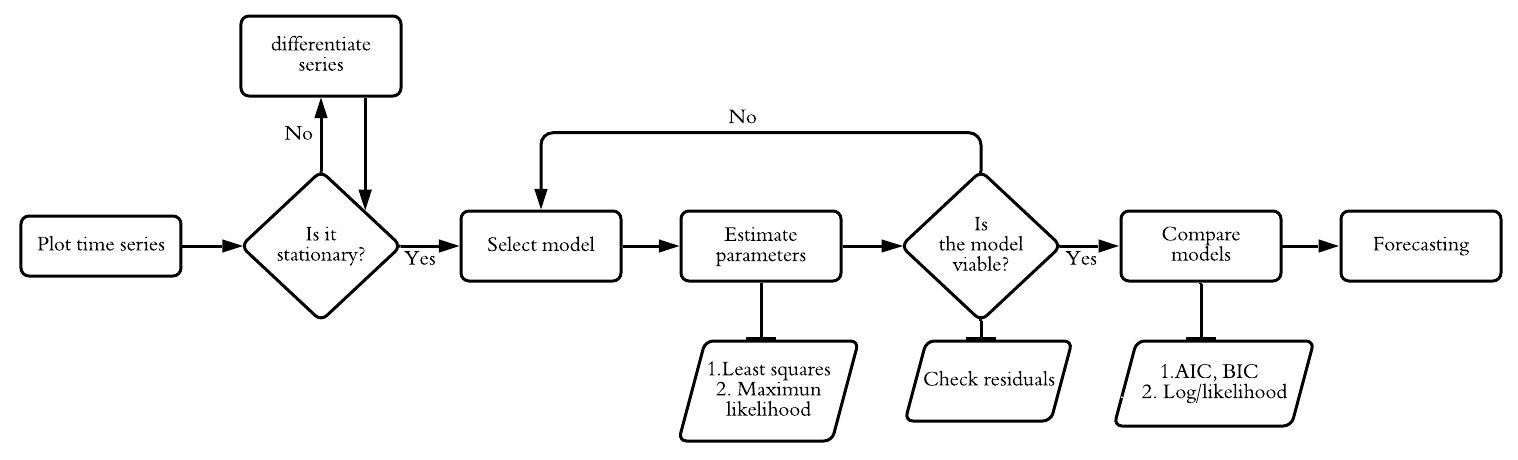
\includegraphics[scale=0.55]{Figs/BJ4}
	\caption{Box-Jenkins methodology (1970).The flow diagram presents the procedure to be used for an adequate data analysis in a frequentist approach, for a further description of said methodology, review \cite{box}.}
	\label{fig:Box}
\end{figure}
%
\begin{enumerate}
	%\item \textit{Data visualization:} la visualización mediante gráficos, permite detectar patrones como  tendencia, estacionalidad, ciclos u observaciones atípicas, que deben ser filtrados diferenciando la serie  o  aplicando diferencias estacionales. Los gráficos ACF (función de autocorrelación)\citet{acf} y PACF (función de autocorrelación parcial) \citet{acf} son de gran importancia para seleccionar los ordenes del modelo \citet{rob}.
	\item \textit{Data visualization:} visualization through graphs allows the detection of patterns such as trends, seasonality, cycles or atypical observations, which must be filtered by differentiating the series or applying seasonal differences. The graphs ACF (autocorrelation function) \citet{acf} and PACF (partial autocorrelation function) \citet{acf} are of great importance to select the orders of the model \citet{rob}.
	
	%\item \textit{Selección:} para definir un modelo inicial es necesario establecer los valores $p,d,q,P,D,Q$ y $m$. Lo valores $d, D$ son el número de diferencias necesarias para que la serie sea estacionaria o un ruido blanco, esto se logra graficando la serie original y la serie diferenciada. Los valores $(p,P)$ y $(q,Q)$  se identifican con los gráficos PACF y ACF respectivamente, como el número de retardos (lags) diferentes de cero en la serie diferenciada, para más detalles ver \cite{rob}.
	\item \textit{Model selection: }to define an initial model it is necessary to establish the values $ p, d, q, P, D, Q $ and $ m $. The values $ d, D $ are the number of differences necessary for the series to be stationary or a white noise, this is achieved by graphing the original series and the differentiated series. The values $ (p, P) $ and $ (q, Q) $ are identified with the graphs PACF and ACF respectively, as the number of lags different from zero in the differentiated series, for more details see \cite{rob}.
	
	%\item \textit{Estimación:} una vez se ha definido un modelo inicial, es necesario estimar los $n_p=p+P+q+Q+2$ parámetros, los métodos más usados son: \textit{mínimos cuadrados} \citet{MLE}, \textit{máxima verosimilitud}\citet{MLE}, y la \textit{ecuación de Yule-Walker} \citet{yule1,yule2}.
	\item \textit{Parameter estimation:} once an initial model has been defined, it is necessary to estimate the $ n_p = p + P + q + Q + 2 $ parameters, the most used methods are:\textit{ least squares} \citet{MLE}, \textit{maximum likelihood} \citet{MLE}, and the \textit{Yule-Walker equation} \citet{yule1,yule2}.
	
	%\item \textit{Diagnóstico:} Los modelos $SARIMA$ siguen el supuesto que los errores siguen un ruido blanco Gaussiano, es decir, los errores son estacionarios con distribución normal. Para diagnóstico de estacionaridad, se utilizan las pruebas de Portmanteau \cite{test} y  Lijung-Box \citet{Lijung-test}, o pruebas de raíz unitaria como la prueba Augmented Dickey-Fuller \citet{ADF}, Phillips-Perron \citet{ADF}, y KPSS \citet{KPSS}. Para medir normalidad pruebas como Epps \citet{Epps}, Lobato-Velasco \citet{LV} y proyecciones aleatorias \citet{rp} que miden normalidad en procesos estacionarios son las más adecuadas. Para más detalles ver \citet{nortstest}.
	\item \textit{Model checking:} the \textit{SARIMA} models follow the assumption that the errors follow a Gaussian white noise, that is, the errors are stationary with normal distribution. For diagnosis of stationarity, the Portmanteau \cite{test} and Lijung-Box tests \citet{Lijung-test} are used, or unit root tests such as the Augmented Dickey-Fuller \citet{ADF}, Phillips-Perron \citet{ADF}, and KPSS tests \citet{KPSS}. To measure normality tests such as Epps \citet{Epps}, Lobato-Velasco \citet{LV} and random projections \citet{rp} that measure normality in stationary processes are the most appropriate. For more details see \citet{nortstest}.
	
	%\item \textit{Comparación:} El criterio de selección de modelos más utilizado es el \textit{Akaike’s Information Criteria (AIC)} propuesto por Akaike en 1974 \citet{akaike}. Sea $n_p=p+q+P+Q+2$ el número de parámetros estimados en el modelo, luego se eligen los valores de $p,q,P,Q$ que minimicen el AIC:
	\item \textit{Model comparison: }the most widely used model selection criterion is the \textit{Akaike’s Information Criteria (AIC)} proposed by Akaike in 1974 \citet{akaike}. Let $ n_p = p + q + P + Q + 2 $ be the number of parameters estimated in the model, then the values of $ p, q, P, Q $ that minimize the AIC are chosen:
	%
	\begin{equation}
		AIC = -2log L+2n_p,
	\end{equation}
	%
	%donde $L$ denota la verosimilitud. Existen varias modificaciones del AIC que también son usadas como el BIC (Bayesian Information Criteria) y la log-verosimilitud. 
	where $L$ denotes the likelihood. There are several modifications of the AIC that are also used as the BIC (Bayesian Information Criteria) and the log-likelihood.
	
	%\item \textit{Predicción:} Una vez elegido el modelo que mejor se ajuste a cada una de las pruebas anteriores se procede a hacer la predicción de las observaciones futuras.
	\item \textit{Forecasting: }once the model that best fits each of the previous tests has been chosen, the prediction of future observations is made.
\end{enumerate}
%
\subsection{Bayesian inference}
%En un enfoque de inferencia Bayesiano, se analiza la probabilidad de un parámetro $\theta \in \Theta$ dada la muestra obtenida $y$, donde $\Theta$ es un espacio de probabilidad para el conjunto de parámetros. Para eso, debemos iniciar por establecer un modelo que proviene de una distribución de probabilidad conjunta para $\theta$ y $y$. La función de probabilidad conjunta puede ser escrita como el producto de dos densidades:
In a Bayesian inference approach, the probability of a parameter $\theta \in \Theta$ is analysed given the sample obtained $y$, where $\Theta$ is a probability space for the set of parameters. For that, we must start by establishing a model that comes from a joint probability distribution for $\theta$ and $y$. The joint probability function can be written as the product of two densities:
%
\begin{equation*}
	p(\theta,y)=p(\theta)p(y|\theta)
\end{equation*}
%
%donde a $p(\theta)$ se le llama la distribución a \textit{priori} y a $p(y|\theta)$ la distribución de la muestra o \textit{verosimilitud}. Al condicionar el valor conocido de los datos $y$ y usando el Teorema de Bayes obtenemos la distribución a \textit{posteriori}:
where $p(\theta)$ is called the \textit{prior} distribution and $p(y|\theta)$ the sample distribution or \textit{likelihood}. By conditioning the known value of the data $y$ and using Bayes Theorem we obtain the \textit{posterior} distribution:
%
\begin{equation*}
	p(\theta|y)=\frac{p(\theta,y)}{p(y)}=\frac{p(\theta)p(y|\theta)}{p(y)}
\end{equation*}
%
%Una forma equivalente de la ecuación anterior omite el factor $p(y)$ el cual, al no depender de $\theta$ se considera una constante, lo que resulta en una distribución posteriori no normalizada, en otras palabras la posteriori es proporcional a la verosimilitud y priori, mediante la siguiente ecuación:
An equivalent form of the previous equation omits the factor $p(y)$ which, as it does not depend on $\theta$ is considered a constant, resulting in a non-normalized posterior distribution, in other words the posterior is proportional to the likelihood and prior, using the following equation:
%
\begin{equation}\label{eq: bayes2}
	p(\theta|y)\propto p(\theta)p(y|\theta)
\end{equation}
%Note que $p(y|\theta):\Theta \to \mathbb{R}$ es una función de $\theta$ cuando la muestra $y$ es fija, y se le conoce como \textit{función de verosimilitud.} Estas ecuaciones bastan para realizar inferencia Bayesiana en donde primero se establece un modelo $p(\theta,y)$ y luego se desarrollan los cálculos computacionales para obtener $p(\theta|y)$ el cual funciona como la información actualizada de los datos. 

%Por otro lado, al inferir observaciones desconocidas o predicciones, seguimos un procedimiento similar. Después de inferir nuestros parámetros $\theta$ a partir de los datos observados $y$, podemos predecir una observación desconocida $\Tilde{y}$. La distribución de $\Tilde{y}$ se conoce como la \textit{distribución predictiva a posteriori} y se obtiene con la siguiente ecuación:
Note that $p(y|\theta):\Theta \to \mathbb{R}$ is a function of $\theta$ when the sample $y$ is fixed, and is known as a \textit{likelihood function.} These equations are enough to perform Bayesian inference where first a model $p(\theta,y)$ is established and then the computational calculations are developed to obtain $p(\theta|y)$ which works as the updated information of the data.

On the other hand, when inferring unknown observations or predictions, we follow a similar procedure. After inferring our parameters $\theta$ from the observed data $y$, we can predict an unknown observation $\tilde{y} $. The distribution of $\tilde{y}$ is known as the \textit{posterior predictive distribution} and is obtained with the following equation:
%
\begin{equation*}
	p(\Tilde{y}|y)=\int p(\Tilde{y},\theta|y)d\theta =\int p(\Tilde{y}|\theta)p(\theta|y)d\theta
\end{equation*}
%
\subsection{Bayesian SARIMA models} \label{sarimab}
%En base a la definiciones previas, se define un \textit{modelo SARIMA Bayesiano} como un modelo ARIMA estacional y una selección de prioris independientes entre si para cada uno de los parámetros desconocidos, siguiendo las siguientes ecuaciones:
Based on the previous definitions, a \textit{Bayesian SARIMA model} is defined as a seasonal ARIMA model and a selection of independent priors for each of the unknown parameters, following the equations:
%
$$y \sim SARIMA(p,d,q)_\times(P,D,Q)_m$$
\begin{align*}
	\phi_i \sim p(\phi_i),& \hspace{0.3cm} i=1,...,p\\
	\theta_j \sim p(\theta_j),& \hspace{0.3cm} j=1,...,q\\
	\Phi_k \sim p(\Phi_k),& \hspace{0.3cm} k=1,...,P\\
	\Theta_w \sim p(\Theta w),& \hspace{0.3cm} w=1,...,Q
\end{align*}
$$\mu_0 \sim p(\mu_0)$$
$$\sigma_0 \sim p(\sigma_0)$$
%
%Donde los datos $y$ son una realización de un proceso estocástico que siguen la ecuación~\eqref{eq:SARIMA}, y $\theta = (\phi_1,\ldots,\phi_p,\theta_1,\ldots,\theta_q,\Phi_1,\ldots,\Phi_P,\Theta_1,\ldots,\Theta_Q,\mu_0,\sigma_0) \in \mathbb{R}^{n_p}$ es el vector de parámetros desconocidos.
Where the data $ and $ are a realization of a stochastic process that follow the equation~\eqref{eq:SARIMA}, y $\theta = (\phi_1,\ldots,\phi_p,\theta_1,\ldots,\theta_q,\Phi_1,\ldots,\Phi_P,\Theta_1,\ldots,\Theta_Q,\mu_0,\sigma_0) \in \mathbb{R}^{n_p}$ is the vector of unknown parameters.
%
\begin{figure}
	\centering
	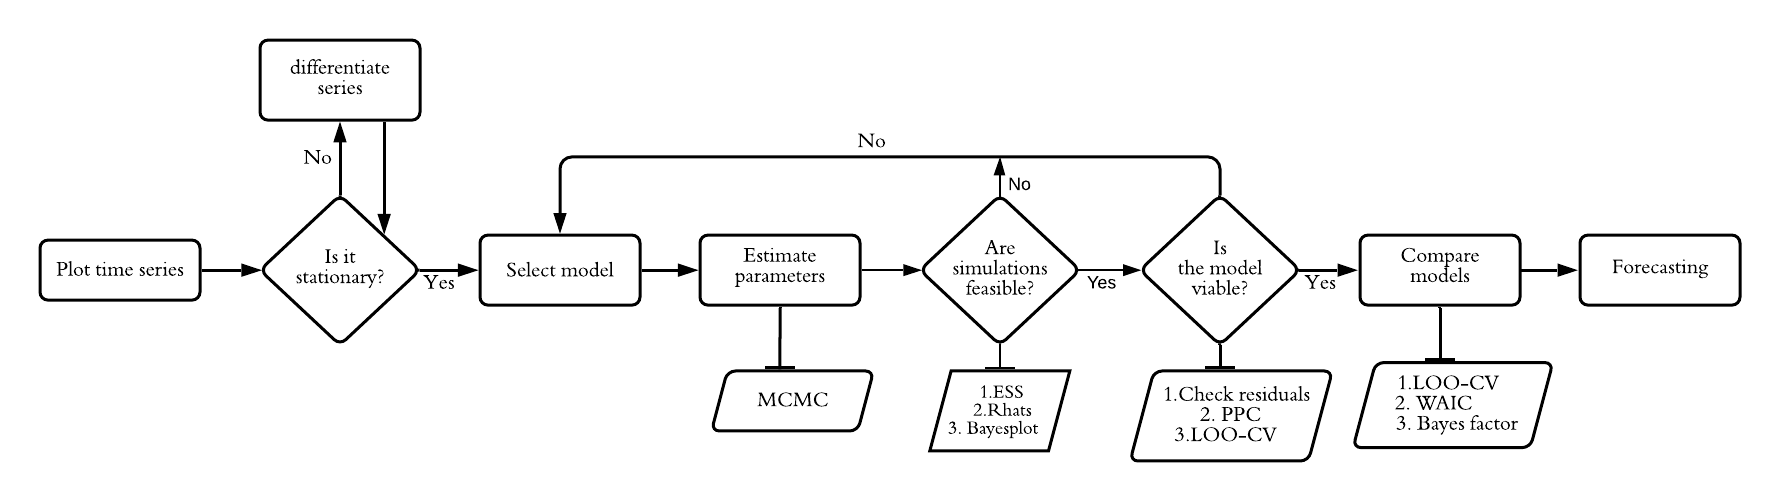
\includegraphics[scale=0.5]{Figs/BBJ1}
	\label{fig:BBJ1}
	\caption{Methodology for prediction with Bayesian SARIMA models. The flow diagram presents the adaptation of the Box-Jenkins method adapted to a Bayesian approach based on the Bayesian workflow proposed by \citet{Aki}.}
\end{figure}
%
\section{Adaptations to the Box-Jenkins method}
%Al proponer un modelo SARIMA Bayesiano para hacer la predicción debemos hacer modificaciones y adaptaciones al Método Box-Jenkins, esto dado que las estimaciones y diagnósticos de parámetros se basan en inferencia Bayesiana. Inicialmente los pasos de \textit{visualización de datos} y \textit{selección del modelo} se mantienen igual, por lo que en las siguientes secciones se expondrán los pasos de \textit{selección, diagnóstico y comparación de los modelos} que se verán modificados siguiendo la linea del \textit{Bayesian Workflow} adaptado al análisis de series temporales.
When proposing a Bayesian SARIMA model to make the forecasting, we must make modifications and adaptations to the Box-Jenkins method, this given that the parameter estimation and checking are based on Bayesian inference. Initially the \textit{data visualization} and \textit{model selection} steps remain the same, so the following sections will show the \textit{selection, checking and comparison of the models} steps that will be seen modified following the line of the \textit{Bayesian Workflow} adapted to the analysis of time series.
%
\subsection{Model estimation}
%Una vez establecido el modelo inicial, y las distribuciones a priori de cada uno de los parámetros, se aproxima la distribución a posteriori mediante Monte Carlo Hamiltoneano el cual simula una cadena de markov estacionaria que converge a la distribución de cada uno de los parámetros. Para una mejor compresión de este proceso de inferencia se recomienda leer \cite{BDA}.
Once the initial model is established and the prior distributions of each parameters, the posterior distribution is approximated by Hamiltonian Monte Carlo which simulates a stationary markov chain that converges to the distribution of each parameter. For a better understanding of this inference process it is recommended to read \cite{BDA}.
%
\subsection{Inference evaluation}
%Luego de hacer la inferencia es necesario evaluar la convergencia de las simulaciones midiendo la estacionaridad y combinación de las cadenas simuladas para cada uno de los parámetros. De esta manera, para decidir la viabilidad de los resultados se utilizarán dos estadísticos, el Tamaño de muestra efectiva \textit{(Effective Sample Size ESS)} y la Reducción de escala potencial (\textit{potencial scale reduction} $\hat{R}$), el primero indica el tamaño suficiente de las simulaciones para aproximar correctamente los parámetros y el segundo es un indicador de convergencia de las cadenas que para este estudio se tomará como estimador factible si $\hat{R}<1.1$. Las propiedades generales de ambos estimadores se encuentran en \cite{BDA}.
%
%Es recomendable además, el análisis gráfico del ajuste a cada parámetro, esto es, observar los histogramas y gráficos de las cadenas generadas en busca de indicios de multimodalidad en la distribución de los parámetros y verificar que las cadenas muestren convergencia. Este análisis gráfico se puede realizar con el paquete \textit{bayesplot}  \cite{bayesplot} y se pueden observar ejemplos en el artículo \citet{visualization}.
After making the inference, it is necessary to evaluate the convergence of the simulations by measuring the stationarity and combination of the simulated chains for each of the parameters. In this way, to decide the viability of the results, two statistics will be used, the \textit{(Effective Sample Size ESS)} and the (\textit{Potential scale reduction} $\hat{R}$), the first indicates the sufficient size of the simulations to correctly approximate the parameters and the second is an indicator of convergence of the chains that for this study will be taken as a feasible estimator if $\hat{R}<1.1$. The general properties of both estimators are found in \cite{BDA}.

It is also recommended to do a graphic analysis of the fit to each parameter, that is, to observe the histograms and graphs of the generated chains in search of signs of multimodality in the distribution of the parameters and to verify that the chains show convergence. This graphical analysis can be performed with the \textit{bayesplot} \cite{bayesplot} package and examples can be seen in the article \citet{visualization}.
%
\subsection{Model checking}
%Al igual que en la Metodología Box-Jenkins es recomendable hacer un diagnóstico de los modelos, comprobando que los errores se comporten como un ruido blanco Gaussiano. Por otro lado en la inferencia Bayesiana existen métodos para constatar que el modelo representa efectivamente los datos observados, el principal método es la \textit{Verificación predictiva a posteriori (PPC)  (Box, 1980, Rubin, 1984, Gelman, Meng, y Stern, 1996)}. Si el modelo se ajusta bien, este debería generar datos con el mismo comportamiento de las observaciones. No obstante PPC no es factible en el análisis de series temporales debido a que los supuestos de intercambiabilidad no se cumplen en los datos al ser realizaciones de un proceso estocástico. Para evadir estos problemas se recomienda hacer PPC en los residuos del modelo ($\widehat{\varepsilon_i} = Y_i - \widehat{Y_i}$) los cuales son estacionarios e intercambiables, por lo que muestran condiciones óptimas para la creación de histogramas y obtención de resultados concluyentes.
As in the Box-Jenkins methodology, it is advisable to make a check of the models, checking that the errors behave like a Gaussian white noise. On the other hand, in Bayesian inference, there are methods to verify that the model effectively represents the observed data, the main method is \textit{Posterior predictive check (PPC) (Box, 1980, Rubin, 1984, Gelman, Meng, and Stern , nineteen ninety six)}. If the model fits well, it should generate data with the same behaviour as the observations. However, PPC is not feasible in the analysis of time series because the assumptions of interchangeability are not fulfilled in the data as they are realizations of a stochastic process. To avoid these problems, it is recommended to do PPC on the model residuals ($\widehat {\varepsilon_i}=Y_i-\widehat{Y_i}$) which are stationary and interchangeable, so they show optimal conditions for the creation of histograms and obtaining conclusive results.
%

%Generalmente la PPC es suficiente para encontrar errores en el ajuste del modelo, sin embargo, dado que usamos las observaciones para ajustar el modelo y hacer las evaluaciones es posible que en algunos casos se dejen pasar comportamientos anormales en los datos. Un camino alternativo es hacer el diagnóstico con validación cruzada \textit{Leave-one-out cross-validation (LOO-CV)} en donde una parte de los datos es utilizada para ajustar el modelo y el resto se utiliza para medir la precisión de predicción. En \cite{Aki} se aconsejan tres maneras de abordar la evaluación usando validación cruzada: 1.Verificaciones de calibración utilizando la distribución predictiva de validación cruzada 2. Identificar qué observaciones o grupos de observaciones son más difíciles de predecir 3. Identificar qué tan influyentes son las observaciones particulares, esto es, cuánta información proporcionan además de otras observaciones. Para una mayor comprensión de LOO-CV se recomienda leer \citet{waic}.
Generally, the PPC is sufficient to find errors in the model fit, however, since we use the observations to fit the model and make the evaluations, it is possible that in some cases atypical behaviours are allowed to pass through the data. An alternative way is to make the diagnosis with \textit{Leave-one-out cross-validation (LOO-CV)} where a part of the data is used to fit the model and the rest is used to measure the precision of prediction. In \cite{Aki} three ways of approaching evaluation using cross-validation are advised: 1. Calibration checks using the cross-validation predictive distribution 2. Identify which observations or groups of observations are most difficult to predict 3. Identify how influential are the particular observations, that is, how much information they provide in addition to other observations. For a better understanding of LOO-CV it is recommended to read \citet{waic}.
%
\subsection{Model comparison} 
%En la comparación de modelos Bayesianos frecuentemente se utilizan LOO-CV y el Criterio de Información Watanabe-Akaike, WAIC (Watanabe, 2010). Ambos métodos estiman la precisión puntual en la predicción en un modelo usando una muestra de la log-verosimilitud. No obstante, el método de estimación de precisión para modelos en series de tiempo que mejores estimaciones propone es la validación cruzada de series de tiempo \citet{cv-time}, pero debido a la dificultad de implementación en este estudio se trabajará con LOO-CV y WAIC solamente.  La implementación de estos métodos se puede realizar con el paquete \textit{loo} \citet{loo_package}. Para una mayor comprensión de los mismos se recomienda leer \citet{loo,waic}.
In the comparison of Bayesian models, LOO-CV and the Watanabe-Akaike Information Criterion, WAIC (Watanabe, 2010) are frequently used. Both methods estimate the point precision in the prediction in a model using a log-likelihood sample. However, the method for estimating precision for time series models that proposes the best estimates is the cross-validation of time series \citet{cv-time}, but due to the difficulty of implementation in this study we will work with LOO-CV and WAIC only. The implementation of these methods can be done with the \textit{loo} \citet{loo_package} package. For a better understanding of them, it is recommended to read \citet{loo, waic}.

%Finalmente, luego de elegir los modelos que presenten mejores resultados en las pruebas anteriores se proceden a hacer la predicciones con los modelos seleccionados. Las herramientas propuestas ofrecen la precisión suficiente para una buena estimación y selección de modelos, sin embargo, hace falta un análisis cuidadoso a la hora de hacer predicciones de valores futuros. En las siguientes secciones se mostrarán ejemplos con datos reales, aplicando nuestra metodología propuesta para seleccionar el modelo SARIMA que mejor se ajuste a los datos en un enfoque Bayesiano.
Finally, after choosing the models that present better results in the previous tests, the predictions are made with the selected models. The proposed tools offer sufficient precision for a good estimation and selection of models, however, careful analysis is required when making predictions of future values. The following sections will show examples with real data, applying our proposed methodology to select the SARIMA model that best fits the data in a Bayesian approach.
%
\section{Illustrations}
%Aplicaremos la nueva metodología estudiando dos conjuntos de datos y realizando sus respectivas predicciones. Para la inferencia y análisis de los modelos  utilizaremos el paquete \textit{bayesforecast} que implementa dichos modelos usando un Monte-Carlo Hamiltoneano, generando 4 cadenas de 2,000 iteraciones y un warm-up de 1,000 iteraciones. Como diagnóstico de convergencia usaremos el estadístico $\hat{R}$ \cite{BDA} y la comparación de los modelos será con validación cruzada usando el paquete $\textit{loo}$ \citet{waic}.
We will apply the new methodology by studying two data sets and making their respective predictions. For the inference and analysis of the models we will use the \textit{bayesforecast} package that implements these models using an Hamiltonian Monte Carlo, generating 4 chains of 2,000 iterations and a warm-up of 1,000 iterations. As a convergence diagnosis we will use the statistic $\hat{R}$ \cite{BDA} and the comparison of the models will be with cross-validated using the $\textit{loo}$ \citet{waic} package.
%
\subsection{Average temperature in Honduras}
%El primer conjunto de datos muestra la temperatura promedio mensual en Honduras  desde el año 1980 hasta el 2013, con un total de 405 observaciones en donde las primeras 385 servirán como conjunto de entrenamiento del modelo y el resto será el conjunto de prueba. Estos datos fueron obtenidos de \textit{Berkeley Earth} \cite{berkeley}.
The first data set shows the monthly average temperature in Honduras from 1980 to 2013, with a total of 405 observations where the first 385 will serve as the training set of the model and the rest will be the test set. These data were obtained from \textit{Berkeley Earth} \cite{berkeley}.
%
\begin{example*}
> library(bayesforecast)
> library(ggplot2)	

> autoplot(object = train, ylab="Celsius", xlab = "Years",size=1) +
+     theme(panel.background = element_rect(fill = "white", colour = "black",
+                                           size = 1, color = "black"),
+           panel.grid.major = element_blank(),
+           panel.grid.minor = element_blank(),
+           axis.text=element_text(size=12, color = "black"),
+           axis.title=element_text(size=14,family="serif"))
\end{example*}	
%
\begin{figure}[!ht]
	\centering
	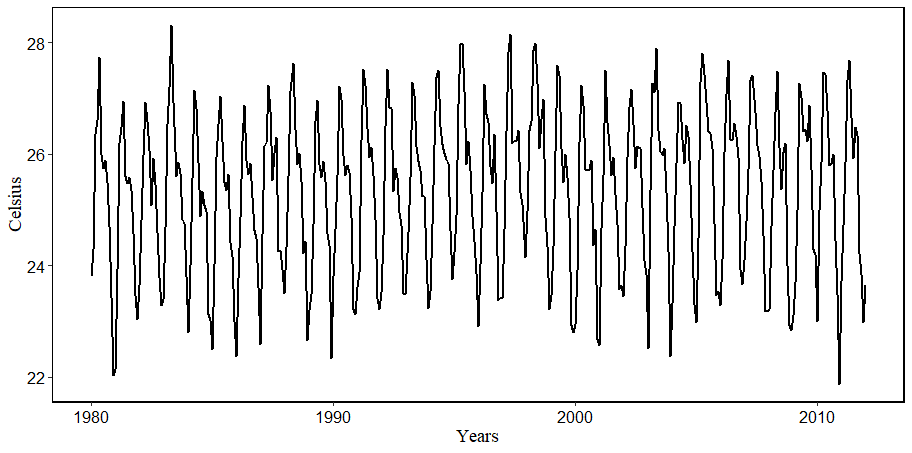
\includegraphics[scale=0.5]{Figs/11}
	\caption{Record of the monthly average temperature in Celsius for Honduras from 1980 to 2013. The series does not present a trend but it does present strong variations and periodic oscillations. Therefore, a seasonal SARIMA model is suitable for the analysis of the series.} \label{fig:temperatura}
\end{figure}
%	

%
%La Figura~\ref{fig:temperatura} muestra que los datos no siguen un comportamiento estacionario, y dado que son observaciones climatológicas se espera que existan patrones estacionales anuales, por lo tanto se aplicará una diferencia estacional con periodo 12 y  una diferencia no estacional.
\begin{example*}
	> head(serie)
	Jan    Feb    Mar    Apr    May    Jun
	1980 23.798 24.296 26.346 26.595 27.735 25.984
\end{example*}

Figure~\ref{fig:temperatura} shows that the data do not follow a stationary behaviour, and since they are climatological observations it is expected that there will be annual seasonal patterns, therefore a seasonal difference with period 12 and a non-seasonal difference will be applied.
%
\begin{example*}
	library(cowplot)
	
	g1 = cbind("Seasonally\n differenced" = diff(train, 12),
	"Doubly\n differenced" = diff(diff(train, 12))) %>%
	autoplot(facets = TRUE) + xlab("Years") + ylab("") 
	
	g2 = ggacf(y = diff(train)) 
	
	g3 = ggpacf(y = diff(train)) 
	
	g4 = plot_grid(g2,g3, labels = NULL)
	plot_grid(g1, g4, labels = NULL, ncol = 1, rel_heights = c(1.3,1))
\end{example*}
\begin{figure}[ht!]
	\centering
	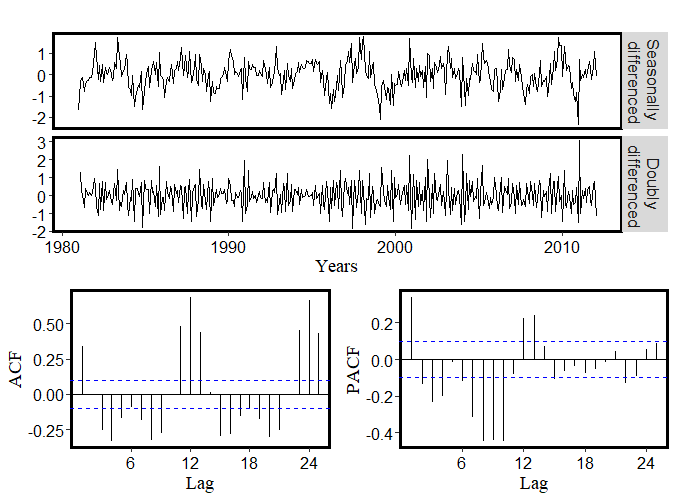
\includegraphics[scale=0.6]{Figs/44}
	\caption{The upper graph shows the series with a seasonal difference with period 12 and then non-seasonally differentiated. The lower graphs show the ACF and PACF functions of the doubly differentiated data.}
	\label{fig:dif}
\end{figure}
%La Figura~\ref{fig:dif} muestra que al aplicar una diferencia estacional la serie de la parte superior no luce estacionaria dado que la media no es constante, sin embargo la estacionalidad se reduce, lo que indica que basta hacer una segunda diferencia no estacional. El gráfico intermedio muestra la serie doblemente diferenciada y esta parece tener una media constante en cero y varianza estable. Al observar las funciones de autocorrelación (ACF) y autocorrelación parcial (PACF) de la parte inferior de la Figura~\ref{fig:dif},  estas muestran una leve correlación de a lo más dos retardos en los datos, el orden del modelo SARIMA inicial a considerar entonces es $p=2$, $d=1$, $q=2$. Por otra parte, ambos gráficos muestran ciertos patrones periódicos y los retardos indican una posible componente autorregresiva estacional, por lo tanto, el orden de la componente estacional es $P = 2$, $D = 1$, $Q = 0$. Finalmente, consideramos las distribuciones a priori de cada uno de los parámetros, en este caso seleccionamos prioris poco informativas. De esta manera el modelo completo es:
Figure~\ref{fig:dif} shows that when applying a seasonal difference the series in the upper part does not look stationary since the mean is not constant, however the seasonality is reduced, which indicates that it is enough to make a second difference not seasonal. The middle graph shows the doubly differentiated series and this appears to have a constant mean at zero and a stable variance. When observing the autocorrelation (ACF) and partial autocorrelation (PACF) functions of the lower part of Figure~\ref{fig:dif}, they show a slight correlation of at most two lags in the data, the order of the initial SARIMA model to consider then is $p = 2$, $d = 1$, $q=2$. On the other hand, both graphs show certain periodic patterns and the lags indicate a possible seasonal autoregressive component, therefore the order of the seasonal component is $P=2$, $D=1$, $Q=0$. Finally, we consider the prior distributions of each of the parameters, in this case we select priors that are not very informative. In this way the complete model is:

$$\text{Model 1} \sim SARIMA(2,1,2)_\times(2,1,0)_{12}$$
$$ \mu_0 \sim t(0,2.5,6)$$
$$ \sigma_0 \sim t(7)$$
$$ ar_i, ma_i \sim N(0,0.5) \hspace{0.3cm} i=1,2$$
$$sar_i \sim N(0,0.5) \hspace{0.5cm} i=1,2$$
%En la Cuadro~\ref{tab:resumen} se muestra un resumen de las distribuciones a posteriori de cada uno de los parámetros. El estadístico $\hat{R}$ de cada uno de ellos indica que las cadenas convergen,  y  los tamaños de muestra efectivo (ESS) son valores mayores al número total de iteraciones, indicando un tamaño de muestra factible para la representación efectiva de los parámetros, por lo tanto, aceptamos la aproximación de las posterioris obtenidas.
Table~\ref{tab:summary} shows a summary of the posterior distributions of each of the parameters. The statistic $\hat{R}$ of each of them indicates that the chains converge, and the effective sample sizes (ESS) are values greater than the total number of iterations, indicating a feasible sample size for the effective representation of the parameters, therefore, we accept the approximation of the obtained posteriors.
%
\begin{table}[!ht]
	\centering
	\begin{tabular}{lcccccc}
		\hline
		& mean & SE & 5\% & 95\% & ESS & $\hat{R}$ \\ 
		\hline
		$\mu_0$ & 0.01 & 0.00 & -0.01 & 0.03 & 3904.71 & 0.9998 \\ 
		$\sigma_0$ & 0.51 & 0.00 & 0.48 & 0.54 & 3489.52 & 0.9999 \\ 
		ar.1 & -0.00 & 0.00 & -0.13 & 0.13 & 4122.60 & 0.9998 \\ 
		ar.2 & -0.02 & 0.00 & -0.10 & 0.06 & 4087.97 & 1.0001 \\ 
		ma.1 & -0.65 & 0.00 & -0.81 & -0.48 & 3967.56 & 0.9998 \\ 
		ma.2 & 0.03 & 0.00 & -0.09 & 0.16 & 3888.24 & 0.9999 \\ 
		sar.1 & -0.68 & 0.00 & -0.77 & -0.60 & 4093.16 & 0.9999 \\ 
		sar.2 & -0.36 & 0.00 & -0.44 & -0.27 & 3934.67 & 0.9998 \\ 
		loglik & -277.24 & 0.03 & -281.00 & -274.51 & 4084.98 & 0.9998 \\ 
		\hline
	\end{tabular}
	\smallskip 
	\caption{Summary of the posterior distributions of each of the parameters for Model 1. The statistics presented are the posterior mean (mean), Standard error (SE), credibility intervals at 90\%, effective sample size (ESS) and the potential scale reduction ($\hat{R}$.) }
	\label{tab:resumen}
\end{table}
%

%En la Figura~\ref{fig:combo} se observa que las cadenas parecen ser estacionarias indicando convergencia, además no se observa multi-modalidad en la distribución a posteriori de los parámetros por lo tanto podemos aceptar las estimaciones del modelo y continuar con el diagnóstico del ajuste en los datos.
In Figure~\ref{fig:combo} it is observed that the chains appear to be stationary indicating convergence, in addition there is no multi-modality in the posterior distribution of the parameters, therefore we can accept the estimates of the model and continue with the checking of fit in data.
%
\begin{figure}[!ht]
	\centering
	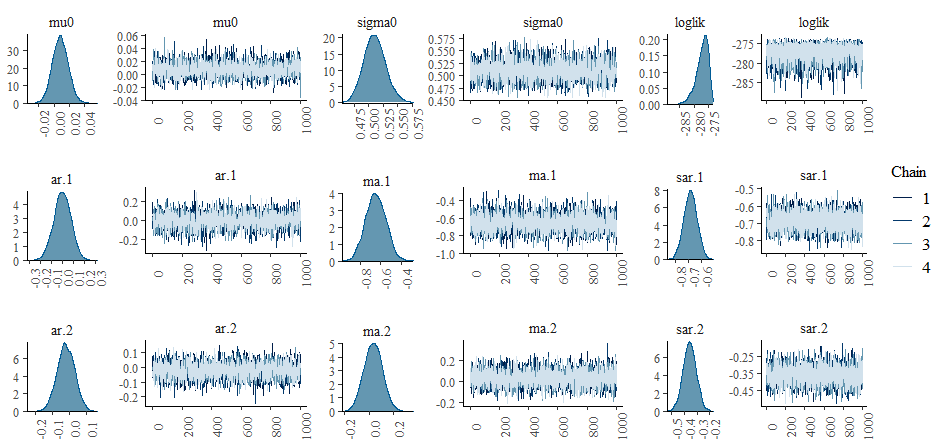
\includegraphics[scale=0.55]{Figs/55}
	\caption{A posterior density graphs and simulated chains for each of the estimated parameters.}
	\label{fig:combo}
\end{figure}
%La Figura~\ref{fig:resi} muestra un resumen de los residuos del modelo 1. El gráfico superior muestra la serie de los residuos, que presenta una leve ciclicidad despreciable y no presenta volatilidad. Los gráficos ACF y PACF en la parte inferior de la Figura~\ref{fig:resi} muestran una baja correlación manteniéndose en los intervalos de confianza por lo tanto, los residuos parecen estacionarios. El histograma y el gráfico de cuantiles (intermedio) muestra que la media a posteriori de los residuos tienen distribución simétrica y sin colas pesadas indicando normalidad. Por lo tanto, concluimos que los residuos siguen un ruido blanco Gaussiano, satisfaciendo los supuestos para el Modelo 1.
Figure~\ref{fig:resi} shows a summary of the residuals of Model 1. The upper graph shows the series of residuals, which presents a slight negligible cyclicality and does not present volatility. The ACF and PACF graphs at the bottom of Figure~\ref{fig:resi} show a low correlation, maintaining the confidence intervals, therefore, the residuals appear stationary. The histogram and the quantile graph (intermediate) show that the posterior mean of the residuals have a symmetric distribution and without heavy tails indicating normality. Therefore, we conclude that the residuals follow a Gaussian white noise, satisfying the assumptions for Model 1.
%
\begin{figure}[!ht]
	\centering
	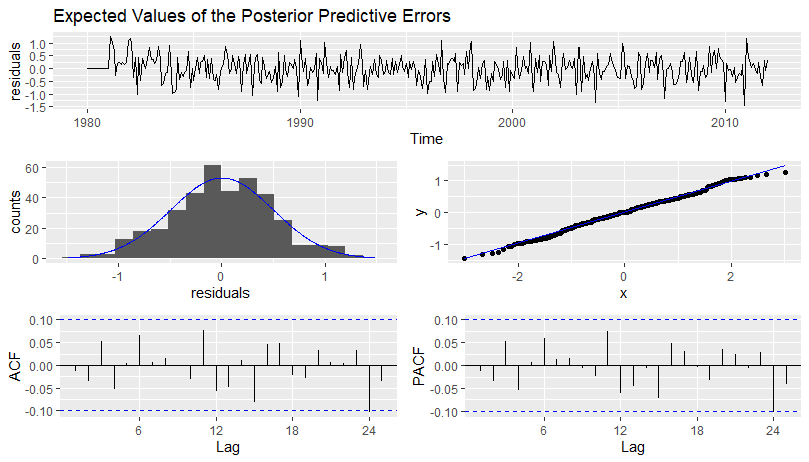
\includegraphics[scale=0.6]{Figs/66}
	\caption{The series of residuals (top). The histogram and quantile graph (middle part). Graphs of autocorrelation and partial autocorrelation of the model residuals (bottom).}
	\label{fig:resi}
\end{figure}
%
\begin{table}[!ht]\centering
	\begin{tabular}{lcc}
		\hline
		& $elpd_{diff}$ & $SE_{diff}$ \\ 
		\hline
		model 1 & 0.00 & 0.00 \\ 
		model 2 & -2.99 & 8.89 \\ 
		model 3 & -29.68 & 12.28 \\ 
		\hline
	\end{tabular}\smallskip 
	\caption{Comparative summary of the precision in each model, where Model 1 shows the best results and Model 3 shows the worst.}\label{tab:loo}
\end{table}
%Comparamos el modelo obtenido con dos modelos alternativos de ordenes diferentes a los propuestos para el modelo inicial, que se definen en las siguientes dos ecuaciones:
We compare the model obtained with two alternative models of different orders to those proposed for the initial model, which are defined in the following two equations:
%
$$\text{Model 2}\sim SARIMA(1,1,0)\times(1,1,1)_{12}$$
$$\text{Model 3}\sim SARIMA(1,0,0)\times(1,1,0)_{12}$$ 
%El Modelo 2 tiene distribuciones a priori ligeramente diferente a los demás modelos, para los parámetros auto-regresivos y de medias móviles (ar,ma, sma) se seleccionó una distribución $Beta(2,2)$ transformada de tal forma que los valores obtenidos estén en el rango $[-1, 1]$, garantizando la estacionaridad del proceso. El resto de los parámetros se mantendrán con las mismas distribuciones que el Modelo 1. Es importante destacar que se utilizó el mismo procedimiento para estimar y diagnosticar los Modelos 2 y 3, validando cada una de las etapas del proceso.
Model 2 has prior distributions slightly different from the other models, for the auto-regressive and moving average parameters (ar, ma, sma) a $Beta(2,2)$ distribution was selected transformed in such a way that the values obtained are in the range $[-1,1]$, guaranteeing the stationarity of the process. The rest of the parameters will remain with the same distributions as Model 1. It is important to note that the same procedure was used to estimate and diagnose Models 2 and 3, validating each of the stages of the process.
%
\begin{figure}[!ht]
	\centering
	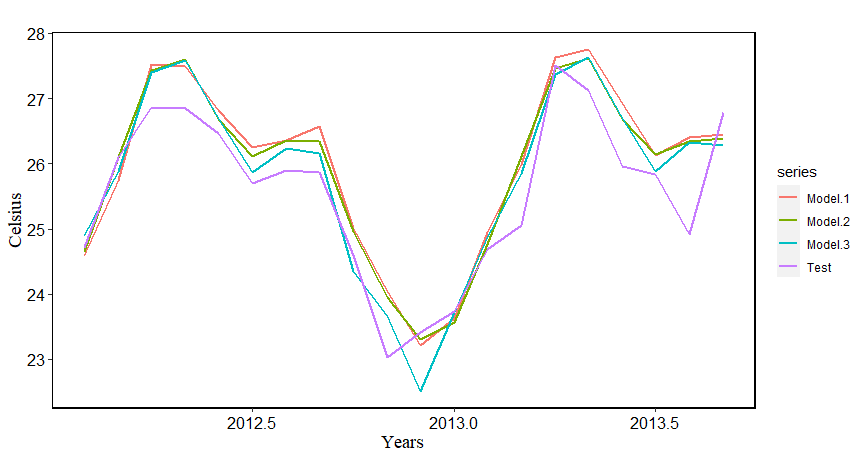
\includegraphics[scale=0.5]{Figs/77}
	\caption{Comparison of predictions of the models with the test set.}
	\label{fig:comp}
\end{figure}
%
\begin{figure}[!ht]
	\centering
	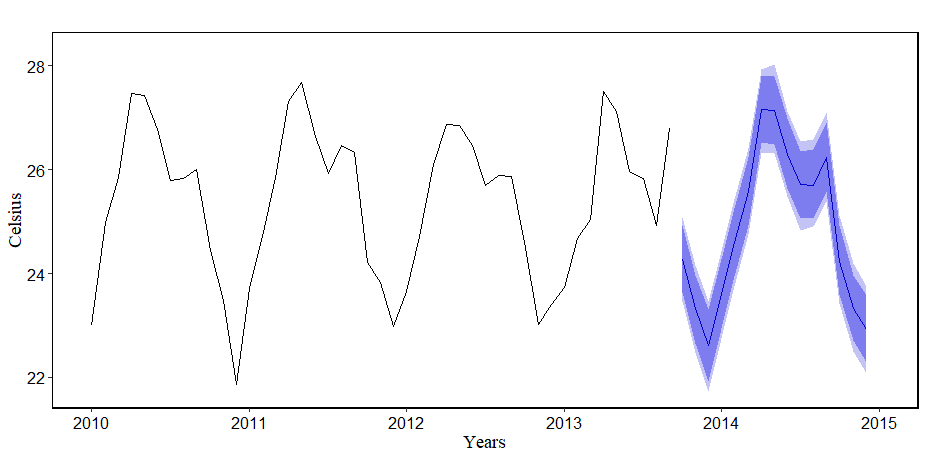
\includegraphics[scale=0.5]{Figs/88}
	\caption{Forecast generated by Model 1.}
	\label{fig:comp}
\end{figure}
%Procedemos a comparar los modelos usando validación cruzada, que estima la medida $elpd$ (Expected log predictive density) para establecer la capacidad predictiva de cada modelo. El Cuadro~\ref{tab:loo}  muestra la diferencia entre $elpds$, donde el Modelo 1 presenta una mayor capacidad predictiva que los otros dos. Adicionalmente, la parte superior de la  Figura~\ref{fig:comp} presenta las predicciones realizadas por cada modelo comparando los resultados con los datos del conjunto de prueba, se observa que cada uno de los modelos generan predicciones muy confiables y similares entre si. Finalmente, seleccionamos el Modelo 1 para predecir los siguientes 15 meses, las predicciones se realizan a partir del mes de Septiembre del año 2013 y los resultados se visualizan en  la parte inferior de la Figura~\ref{fig:comp}.
We proceed to compare the models using cross-validation, which estimates the \textit{elpd} (Expected log predictive density) measure to establish the predictive capacity of each model. Table~\ref{tab:loo} shows the difference between \textit{elpds} , where Model 1 has a higher predictive capacity than the other two. Additionally, the upper part of Figure~\ref{fig:comp} presents the predictions made by each model comparing the results with the data of the test set, it is observed that each of the models generate very reliable predictions that are similar to each other. Finally, we select Model 1 to predict the next 15 months, the predictions are made from the month of September 2013 and the results are displayed in the lower part of Figure~\ref{fig:comp}.
%
\subsection{Closing price on Pfizer stocks}
%Para el segundo ejemplo estudiamos el precio de cierre de las acciones en la empresa farmacéutica Pfizer, en este caso el conjunto de datos es obtenido de \citet{kaggle}, la data muestra los atributos principales de las acciones desde junio de 1972 hasta septiembre de 2021 con 4 mediciones mensuales. Por conveniencia analizaremos el promedio mensual del precio de cierre desde enero del 2010. La serie final con que trabajaremos consta de 141 observaciones, en donde las primeras 134 será el conjunto de entrenamiento y el resto el conjunto de prueba. 
For the second example we study the closing price of the stocks in the pharmaceutical company Pfizer, in this case the data set is obtained from \citet{kaggle}, the data shows the main attributes of the shares from June 1972 to September 2021 with 4 monthly measurements. For convenience, we will analyse the monthly average of the closing price since January 2010. The final series with which we will work consists of 141 observations, where the first 134 will be the training set and the rest the test set.
%
\begin{figure}
	\centering
	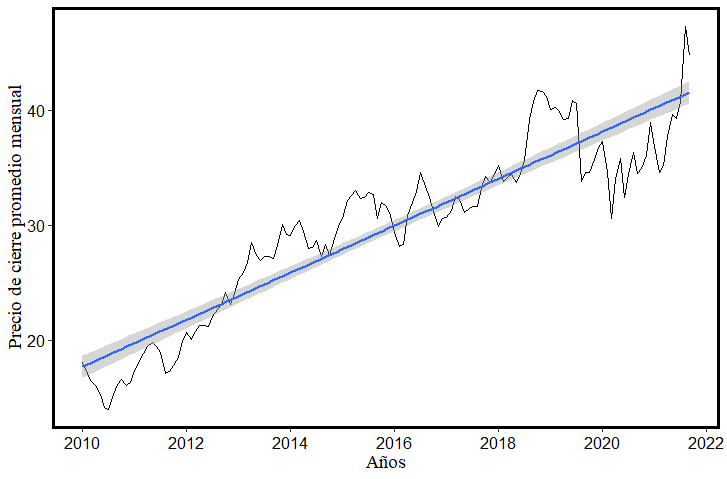
\includegraphics[scale=0.5]{Figs/a}
	\caption{Average closing price in dollars from January 2010 to September 2021.}
	\label{fig:clousure}
\end{figure}
%La  Figura~\ref{fig:cierre} muestra que los datos poseen tendencia creciente que se modela con un modelo SARIMA con tendencia determinista \citet{regresion}.
Figure~\ref{fig:clousure} shows that the data have an increasing trend that is modeled with a SARIMA model with deterministic trend \citet{regresion}.
%
\begin{figure}
	\centering
	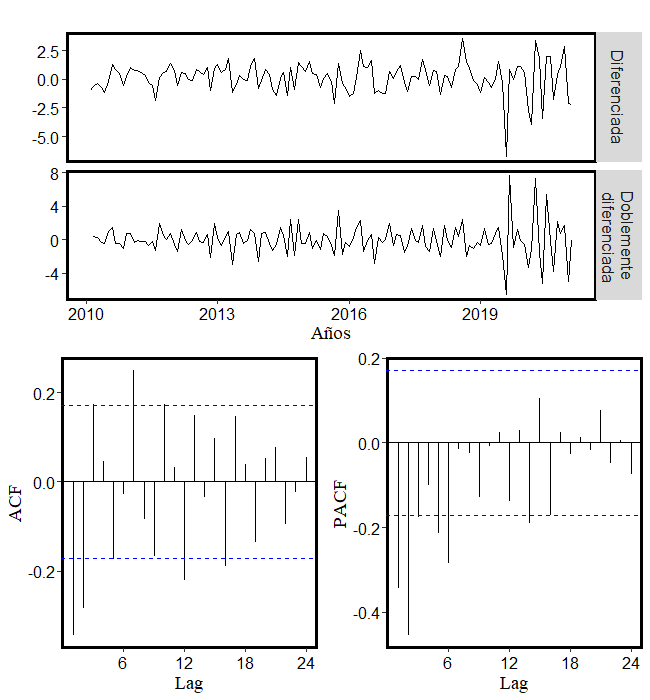
\includegraphics[scale=0.5]{Figs/b}
	\caption{The upper graphs show the non-seasonally differentiated and doubly differentiated data. The lower graphs show the graphs of the ACF and PACF of the doubly differentiated data.}
	\label{fig:acf2}
\end{figure}
%
%Por otra parte, en la Figura~\ref{fig:acf2} observamos que los datos se estabilizan desde la primera diferencia, además es importante notar la alta volatilidad que se presenta en el periodo entre 2019 y 2021. En base a estos hechos y tomando como referencia los gráficos ACF y PACF que indican un posible modelo autorregresivo definiremos el modelo a utilizar:
On the other hand, in Figure~\ref{fig:acf2} we observe that the data stabilizes from the first difference, it is also important to note the high volatility that occurs in the period between 2019 and 2021. Based on these facts and taking as reference the ACF and PACF graphs that indicate a possible autoregressive model, we will define the model to be used:
%
$$\text{Model 1: } y_t = \beta_1 t+\eta_t$$
$$\eta_t \sim SARIMA(1,1,0)_\times(1,0,0)_{12}$$
$$ \mu_0 \sim t(0,2.5,6) \text{ , } \beta_1 \sim t(0,2.5,6)$$
$$ \sigma_0 \sim t(7)$$
$$ ar, sar  \sim N(0,0.5)$$
%
%El modelo $y_t$ es una modelo de regresión con sus error $\eta_t$, de esta forma inferimos en cada uno de los parámetros del modelo SARIMA y el parámetro de regresión. En el Cuadro~\ref{tab:resumen2} se muestra un resumen de las distribuciones a posteriori de los parámetros. El estadístico $\hat{R}$ indica convergencia para cada uno de los parámetros, lo cual se confirma visualmente en la Figura~\ref{fig:cadenas2}, los gráficos de las distribuciones a posteriori no muestran multi-modalidad y las cadenas se parecen estacionarias, las cuales en este contexto son condiciones suficientes para suponer que se obtuvo una inferencia factible.
The model $y_t$ is a regression model with its errors $\eta_t$, in this way we infer in each one of the parameters of the SARIMA model and the regression parameter. Table~\ref{tab:resumen2} shows a summary of the posterior distributions of the parameters. The statistic $\hat{R}$ indicates convergence for each of the parameters, which is visually confirmed in Figure~\ref {fig:cadenas2}, the graphs of the posterior distributions do not show multi-modality and the chains seem stationary, which in this context are sufficient conditions to suppose that a feasible inference was obtained.
%
\begin{table}[ht]\centering
	\begin{tabular}{lcccccc}
		\hline
		& mean & SE & 5\% & 95\% & ESS & $\hat{R}$ \\ 
		\hline
		$\mu_0$ & 0.12 & 0.03 & -2.92 & 3.17 & 3548.40 & 1.0012 \\ 
		$\sigma_0$ & 1.32 & 0.00 & 1.20 & 1.47 & 3884.63 & 1.0025 \\ 
		ar & 0.06 & 0.00 & -0.08 & 0.20 & 3738.73 & 1.0004 \\ 
		sar & -0.25 & 0.00 & -0.41 & -0.08 & 4392.88 & 1.0003 \\ 
		$\beta_1$ & 0.02 & 0.03 & -3.03 & 3.07 & 3567.41 & 1.0012 \\ 
		loglik & -225.95 & 0.02 & -228.70 & -224.33 & 3227.89 & 1.0016 \\ 
		\hline
	\end{tabular}\smallskip 
	\caption{Summary of the posterior distributions of each of the parameters for Model 1. The statistics presented are the posterior mean (mean), Standard error (SE), credibility intervals at 90\%, effective sample size (ESS) and the potential scale reduction ($\hat{R}$.)} \label{tab:resumen2}
\end{table}
%
\begin{figure}[ht] \centering
	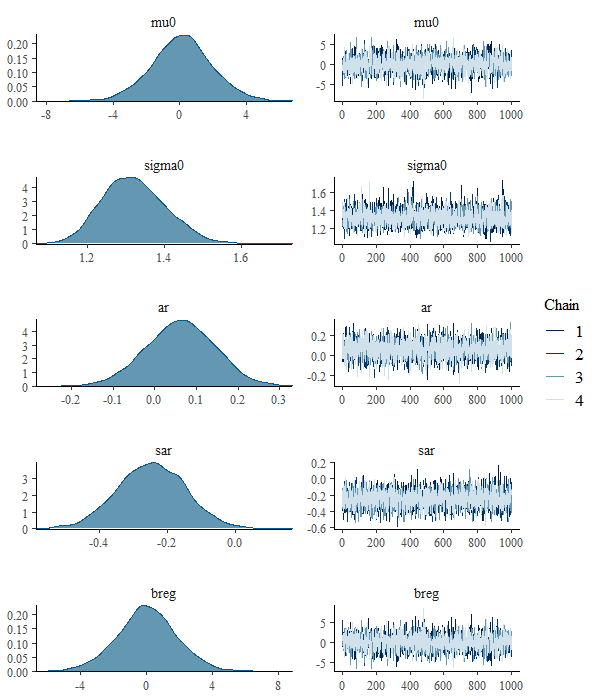
\includegraphics[width = 0.9\columnwidth]{Figs/c.png}
	\caption{Plots of the posterior densities and the simulated chains for each of the estimated parameters.}\label{fig:cadenas2}
\end{figure}
%
%Luego, al observar la Figura~\ref{fig:residuos2} se muestra en la serie de los residuos que el modelo no explica correctamente el periodo entre 2019 y 2021 esto debido a la alta volatilidad en esos años, lo cual también se representa en la gráfica de densidad y cuantiles que muestran presencia de colas pesadas, sin embargo, dada la baja autocorrelación mostradas en los gráficos ACF, PACF y el resto de la serie de los residuos este es un modelo factible para el ajuste de los datos. Por otra parte, los gráficos de autocorrelación muestran que un aumento en el orden del modelo autorregresivo podría mejorar los resultados. 
Then, when looking at Figure~\ref{fig:residuos2} it is shown in the series of residuals that the model does not correctly explain the period between 2019 and 2021 this due to the high volatility in those years, which is also represented in the density graph and quantiles showing the presence of heavy tails, however, given the low autocorrelation shown in the ACF, PACF graphs and the rest of the series of residuals, this is a feasible model for the adjustment of the data. On the other hand, the autocorrelation plots show that an increase in the order of the autoregressive model could improve the results.
%
\begin{figure}[ht]
	\centering
	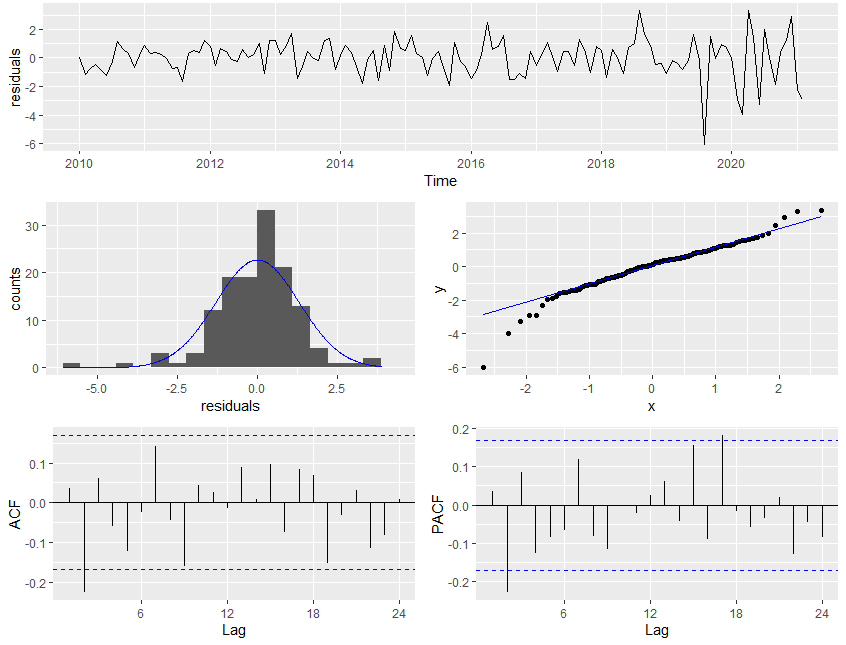
\includegraphics[width = 1\columnwidth]{Figs/d}
	\caption{The series of residuals (top). The histogram and quantile graph (middle part). Graphs of autocorrelation and partial autocorrelation of the model residuals (bottom).}
	\label{fig:residuos2}
\end{figure}
%
%Ahora, en la comparación de modelos se proponen otras dos regresiones con errores ARIMA los cuales son:
Now, in the comparison of models, two other regressions with ARIMA errors are proposed, which are:

$$\text{Model 2: } y_t = \beta_1 t+\eta_t$$
$$\eta_t \sim ARIMA(1,1,0)$$
$$\text{Model 3: } y_t = \beta_1 t+\eta_t$$
$$\eta_t \sim ARIMA(1,0,0)$$
%
%Para el modelo 2, se prueba analizar los datos sin una componente estacional y para el modelo 3 se propone un modelo $AR(1,0,0)$ sin hacer una diferencia  lo que indica que los errores se basan únicamente en el ajuste autorregresivo, por lo que la comparación se basa específicamente en el orden de los errores ya que las distribuciones a priori de los tres modelos son las mismas. La Figura~\ref{fig:comp3} muestra que el Modelo 3 presenta los peores resultados, sin embargo, los Modelos 1 y 2 muestran predicciones similares.
For Model 2, we try to analyse the data without a seasonal component and for Model 3 a component $ AR (1,0,0) $ is proposed without making a difference, which indicates that the errors are based solely on the autoregressive adjustment, so the comparison is based specifically on the order of the errors since the prior distributions of the three models are the same. Figure~\ref{fig:comp3} shows that Model 3 shows the worst results, however, Models 1 and 2 show similar predictions.
%
\begin{figure}[ht]\centering
	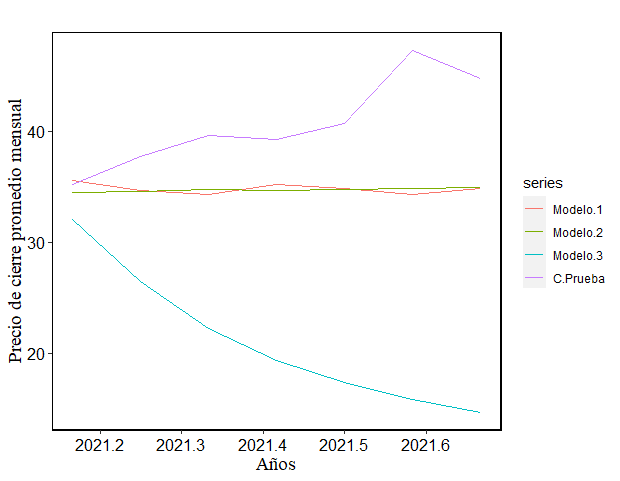
\includegraphics[scale=0.5]{Figs/e}\\
	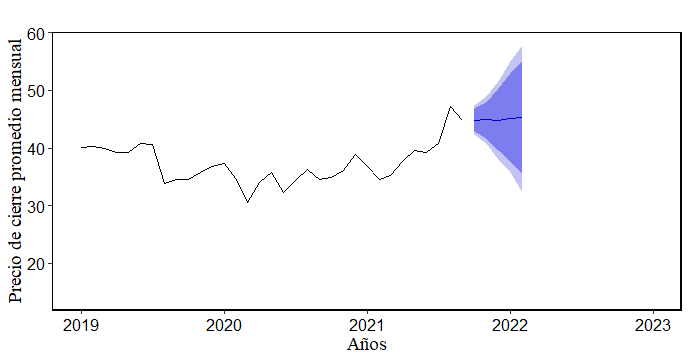
\includegraphics[scale=0.5]{Figs/f}
	\caption{The upper part compares the predictions of the models with the test set. The lower part presents the prediction generated by Model 1, from October 2021 to February 2022.} \label{fig:comp3}
\end{figure}
%Por otro lado, al aplicar CV-LOO y calcular las diferencias de precisión en los modelos se obtiene que el Modelo 1 presenta una mayor precisión que el Modelo 2, por lo tanto se procede a realizar la predicción final mediante el primer modelo. Al observar la Figura~\ref{fig:comp3} se muestra una predicción con comportamiento lineal, sin embargo en el contexto de las observaciones y la tendencia creciente es posible que los valores reales del futuro sean mayores a la predicción obtenida, no obstante, es una buena primera predicción que se puede optimizar mediante la inclusión de variables exógenas.
On the other hand, when applying CV-LOO and calculating the precision differences in the models, it is obtained that Model 1 presents a higher precision than Model 2, therefore the final prediction is made using the first model. Observing Figure~\ref{fig:comp3} shows a prediction with linear behaviour, however, in the context of the observations and the increasing trend, it is possible that the real values of the future are greater than the prediction obtained, however, it is a good first prediction that can be optimized by including exogenous variables.
%
\begin{table}[ht]\centering
	\begin{tabular}{ccc}
		\hline
		& $elpd_{diff}$ & $SE_{diff}$  \\ 
		\hline
		model 1 & 0.00 & 0.00  \\ 
		model 2 & -1.74 & 3.21  \\ 
		model 3 & -47.19 & 35.44 \\ 
		\hline
	\end{tabular}\smallskip 
	\caption{Comparative summary of the precision in each model, where Model 1 shows the best results and model 3 shows the worst.} \label{tab:loo2}
\end{table}
%
\section{Conclusions}
%En este estudio introducimos una nueva metodología para el análisis y predicción de series temporales con modelos SARIMA en un enfoque Bayesiano. La metodología propuesta permite realizar un proceso adecuado de inferencia, diagnostico y selección de modelos, para el análisis de series temporales con modelos SARIMA.
%Hemos presentado el desempeño y aplicabilidad de la metodología mediante dos ejemplos en donde ambos presentaron resultados satisfactorios
In this study we introduce a new methodology for the analysis and prediction of time series with SARIMA models in a Bayesian approach. The proposed methodology allows to carry out an adequate process of inference, checking and selection of models, for the analysis of time series with SARIMA models.
We have presented the performance and applicability of the methodology through two examples where both presented satisfactory results.

\bibliography{daniel-dala}

\address{Daniel Dala\\
  Departamento de Estadística\\
  Universidad Nacional Autónoma de Honduras\\
  Honduras\\
  (ORCiD if desired)\\
  \email{andresht6@hotmail.com}}

\address{Author Two\\
  Affiliation\\
  Address\\
  Country\\
  (ORCiD if desired)\\
  \email{author2@work}}